\documentclass[10pt,xcolor=svgnames]{beamer} %Beamer
\usepackage{palatino} %font type
\usefonttheme{metropolis} %Type of slides
\usefonttheme[onlymath]{serif} %font type Mathematical expressions
\usetheme[progressbar=frametitle,titleformat frame=smallcaps,numbering=counter]{metropolis} %This adds a bar at the beginning of each section.
\useoutertheme[subsection=false]{miniframes} %Circles in the top of each frame, showing the slide of each section you are at

\usepackage{appendixnumberbeamer} %enumerate each slide without counting the appendix
\setbeamercolor{progress bar}{fg=Maroon!70!Coral} %These are the colours of the progress bar. Notice that the names used are the svgnames
\setbeamercolor{title separator}{fg=DarkSalmon} %This is the line colour in the title slide
\setbeamercolor{structure}{fg=black} %Colour of the text of structure, numbers, items, blah. Not the big text.
\setbeamercolor{normal text}{fg=black!87} %Colour of normal text
\setbeamercolor{alerted text}{fg=DarkRed!60!Gainsboro} %Color of the alert box
\setbeamercolor{example text}{fg=Maroon!70!Coral} %Colour of the Example block text


\setbeamercolor{palette primary}{bg=NavyBlue!50!DarkOliveGreen, fg=white} %These are the colours of the background. Being this the main combination and so one. 
\setbeamercolor{palette secondary}{bg=NavyBlue!50!DarkOliveGreen, fg=white}
\setbeamercolor{palette tertiary}{bg=NavyBlue!40!Black, fg= white}
\setbeamercolor{section in toc}{fg=NavyBlue!40!Black} %Color of the text in the table of contents (toc)

%These next packages are the useful for Physics in general, you can add the extras here. 
\usepackage{amsmath,amssymb,amsthm}
\usepackage{slashed}
\usepackage{cite}
\usepackage{relsize}
\usepackage{caption}
\usepackage{subcaption}
\usepackage{multicol}
\usepackage{booktabs}
\usepackage[scale=2]{ccicons}
\usepackage{pgfplots}
\usepgfplotslibrary{dateplot}
\usepackage{geometry}
\usepackage{xspace}
\newcommand{\themename}{\textbf{\textsc{bluetemp}\xspace}}%metropolis}}\xspace}
\graphicspath{{./images/}}

\usepackage{tikz}
\usetikzlibrary{shapes.geometric, arrows}

\tikzstyle{process} = [rectangle, rounded corners, minimum width=2.5cm, minimum height=1cm, text centered, text width=2.3cm, draw=black, fill=orange!30]
\tikzstyle{arrow} = [thick,->,>=stealth]

%%%%%%%%%%%%%%%%%%%%%%%%%%%%%%%%%%%
% CUSTOM function

\newcommand{\R}{\mathbb{R}}
\newcommand{\E}{\mathbb{E}}
\newcommand{\var}{\text{Var}}
\newcommand{\tr}{^{\intercal}}
\newcommand{\med}{\text{med}}
\newcommand{\bb}[1]{\boldsymbol{#1}}




%%%%%%%%%%%%%%%%%%%%%%%%%%%%%%%%%%%%
% GIVE TITLE AUTHOR ETC.

\title{Review of Robust Location and Scatter Estimators}
\author[Name]{Subhrajyoty Roy \inst{$\dagger$} \\ \textbf{Supervisors:} Prof. Ayanendranath Basu and Dr. Abhik Ghosh} %With inst, you can change the institution they belong
%\subtitle{Subtitle}
\institute[uni]{\inst{$\dagger$} External Research Fellow \\ Indian Statistical Institute, Kolkata}
\date{February, 2024} %Here you can change the date
%\titlegraphic{\vspace{-0.5cm}\hfill\includegraphics[scale=0.23]{logo.png}} %You can modify the location of the logo by changing the command \vspace{}. 

%%%%%%%%%%%%%%%%%%%%%%%%%%%%%%%%%%%%%%%%%%%%%%%%%%%%%%%%%%
% BEGIN DOCUMENT HERE
\begin{document}
{
\setbeamercolor{background canvas}{bg=NavyBlue!50!DarkOliveGreen, fg=white}
\setbeamercolor{normal text}{fg=white}
\maketitle
}%This is the colour of the first slide. bg= background and fg=foreground

\metroset{titleformat frame=smallcaps} %This changes the titles for small caps


\begin{frame}{Outline}
  \setbeamertemplate{section in toc}[sections numbered] %This is numbering the sections
  \tableofcontents[hideallsubsections] %You can comment this line if you want to show the subsections in the table of contents
\end{frame}


\section{Introduction}

\begin{frame}{Science built of uncertainty modelling}
    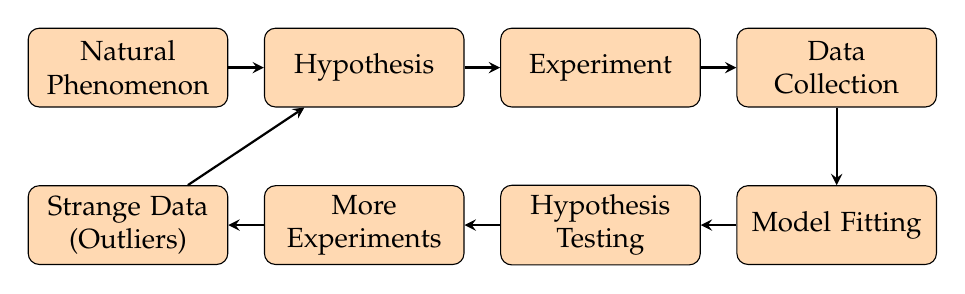
\begin{tikzpicture}[node distance=2cm]
        \node (a1) [process] {Natural \\Phenomenon};
        \node (a2) [process, right of=a1, xshift=1cm] {Hypothesis};
        \node (a3) [process, right of=a2, xshift=1cm] {Experiment};
        \node (a35) [process, right of=a3, xshift=1cm] {Data\\Collection};
        \node (a4) [process, below of=a35] {Model Fitting};
        \node (a5) [process, left of=a4, xshift=-1cm] {Hypothesis\\Testing};
        \node (a6) [process, left of=a5, xshift=-1cm] {More\\Experiments};
        \node (a7) [process, left of=a6, xshift=-1cm] {Strange Data\\(Outliers)};
        \draw [arrow] (a1) -- (a2);
        \draw [arrow] (a2) -- (a3);
        \draw [arrow] (a3) -- (a35);
        \draw [arrow] (a35) -- (a4);
        \draw [arrow] (a4) -- (a5);
        \draw [arrow] (a5) -- (a6);
        \draw [arrow] (a6) -- (a7);
        \draw [arrow] (a7) -- (a2);
    \end{tikzpicture}\\
    \vspace{2cm}
     An \textbf{outlier} is an observation that deviates from the fit suggested by the majority of the data.
\end{frame}

\begin{frame}{Why need robust estimators?}
    \begin{enumerate}
        \item Statistical models are built on assumptions.
        \item Assumptions are often approximations of reality.
        \begin{enumerate}
            \item Fuzzy knowledge.
            \item Outliers, part of data that differs significantly from the majority of it.
        \end{enumerate}
        \item Robust Statistical Inference builds methods that are resistant.
        \item Achieves enough statistical guarantee even when assumptions fail to be met.
    \end{enumerate}
\end{frame}

\begin{frame}{Robustness in Multivariate Context - 1}
    Consider a data matrix
    \begin{equation*}
        \bb{X} = \begin{bmatrix}
            1 & 2 & 3\\
            4 & 5 & 6\\
            \dots & \dots & \dots \\
            13 & 14 & 15
        \end{bmatrix}
    \end{equation*}
    \noindent The singular values of $\bb{X}$ are $35.18, 1.47$ and $0$.\\
    \pause 
    Modification of a single entry $\bb{X}_{11} = 100$ makes the singular values $102.07, 28.62$ and $0.46$.
\end{frame}

\begin{frame}{Robustness in Multivariate Context - 2}
    Coordinatewise \textbf{median} is not a good solution!\\
    \begin{figure}
        \centering
        \includegraphics[width = 0.6\textwidth]{v-data.png}
    \end{figure}
\end{frame}


\begin{frame}{How?}
    Huber defines three desirable features that every robust procedure should achieve. 
    \begin{enumerate}
        \item \textbf{Stability} of the estimator under small deviations from the assumed model.
        \pause
        \item \textbf{Efficiency} under the assumed model.
        \pause
        \item \textbf{Breakdown}-resistance under large amount of contamination.
    \end{enumerate}
\end{frame}

\begin{frame}{General Model}
    Let, $X_1, X_2, \dots X_n$ be an i.i.d sample from $F_{\theta}$, for some unknown $\theta \in \Theta$.\\
    We wish to make inference about $\theta$.\\
    and let, $T(X_1, \dots X_n)$ be the proposed estimator of $\theta$.\\
    We denote $T : \mathcal{F} \rightarrow \R$ as the corresponding functional, i.e.,
    \begin{equation*}
        T(F_n) = T(X_1, \dots X_n),
    \end{equation*}
    \pause
    \textbf{Examples:}
    \begin{enumerate}
        \item For sample mean, $T_1(F) = \int x dF$.
        \item For sample median, $T_2(F) = F^{-1}(1/2)$.
    \end{enumerate}
\end{frame}


\begin{frame}{Fisher Consistency}
    An estimator is \textbf{Fisher consistent} if 
    \begin{equation*}
        T(F_\theta) = \theta,
    \end{equation*}
    \noindent for all $\theta \in \Theta$.\\

    \pause 
    \textbf{Examples:}\\
    \begin{enumerate}
        \item $T(x) = c$, constant \textbf{is not} Fisher consistent.
        \item $T(x) = \left( \int (x - \int x dF)^2 dF \right)^{1/2}$ \textbf{is} Fisher consistent for standard deviation, \textbf{but not} unbiased.
    \end{enumerate}
\end{frame}

\begin{frame}{Influence Function}
    Let, $F_{\epsilon} = (1-\epsilon)F_{\theta} + \epsilon \delta_x$.\\
    Let, $Y_1, \dots Y_n \sim F_{\epsilon}$.\\
    \begin{equation*}
        \text{Empirical } IF(x; T, F_{\theta}) = \lim_{\epsilon \rightarrow 0+}\dfrac{T(Y_1, \dots Y_n) - T(X_1, \dots X_n)}{\epsilon}
    \end{equation*}
    In terms of functional,
    \begin{equation*}
        IF(x; T, F) = \lim_{\epsilon \rightarrow 0+} \dfrac{T((1-\epsilon)F + \epsilon \delta_x ) - T(F)}{\epsilon}
    \end{equation*}
\end{frame}

\begin{frame}{Asymptotic Variance}
    Using Von Mises expansion, one can write
    \begin{align*}
        & T(F_n) = T(F) + \int IF(x; T, F) dF_n(x) + \text{remainder}\\
        \Rightarrow \quad & \sqrt{n}(T(F_n) - T(F)) = \dfrac{1}{\sqrt{n}} \sum_{i=1}^n IF(X_i, T, F) + \text{remainder}\\
        & \text{Under standard regularity assumptions,}\\
        \Rightarrow \quad & \sqrt{n}(T(F_n) - T(F)) \xrightarrow{d} \mathcal{N}\left( 0, \int IF(x; T, F)^2 dF(x) \right)
    \end{align*}
    \pause
    
    \noindent Therefore, the asymptotic variance of centered and normalized estimator $T(F_n)$ is 
    \begin{align*}
        V(T, F) = \int IF(x; T, F)^2 dF(x)
    \end{align*}
\end{frame}

\begin{frame}{Breakdown Point}
    \textbf{Example:} Given a sample $X_1, \dots X_n$ and the estimator sample mean $\bar{X}$, one can modify $X_1$ to make $\bar{X}$ as large (or as small) as required.\\
    In other words, one can break its reliability by contaminating only one sample.\\
    \pause 
    \begin{equation*}
        \epsilon_n^\ast(T; x_1, x_2, \dots x_n) 
        = \dfrac{1}{n} \max\{ m : \max_{i_1, \dots i_m} \sup_{Y_{1}, \dots Y_{m}} T(Z_1, Z_2, \dots Z_n) < \infty \}
    \end{equation*}
    \noindent where $Z_l = X_l$ if $l \notin \{ i_1, \dots i_m \}$ and $Z_l = Y_j$ if $l = i_j$.\\

    \pause
    \noindent \textbf{Asymptotic Breakdown point} is the limit of $\epsilon_n^\ast$ as $n \rightarrow \infty$.
\end{frame} 

\section{Existing Robust Location and Covariance Estimators}

\begin{frame}{Model}
    Let, $X_1, X_2, \dots X_n$ be an i.i.d sample $\sim F(\mu, \Sigma)$, each $X_i \in \R^p$.\\
    
    Also, assume $\E(X_i) = \mu$ and $\var(X_i) = \Sigma$.\\
    
    Both $\mu$ and $\Sigma$ are unknown.\\
    
    We want to estimate these robustly, so that even if some of the $X_i$s come from $G$, such that $G \approx F$, our estimate won't change rapidly.
\end{frame}

\begin{frame}{Trimmed and Winsorized estimator}
    Let, $z_1, z_2, \dots z_n$ be univariate samples.\\
    Since, usual mean is nonrobust, as it has unbounded influence function.\\
    We wish to have a bounded influence for each sample $z_i$.\\
    Let, $z_{(1)} < z_{(2)} < \dots z_{(n)}$ be the order statistics.
    \begin{enumerate}
        \item \text{$\alpha$-Trimmed Estimator:} 
        \begin{equation*}
            \bar{z}_{\alpha} = \dfrac{1}{(n - 2[n\alpha])} \sum_{i=(1+[n\alpha ])}^{n-[n\alpha]} z_{(i)}
        \end{equation*}
        \pause
        \item \text{$\alpha$-Winsorized Estimator:}
        \begin{equation*}
            \bar{z}_{\alpha}^\ast = \dfrac{1}{n} \left( [n\alpha] z_{(1+[n\alpha])} + \sum_{i=(1+[n\alpha ])}^{n-[n\alpha]} z_{(i)} + [n\alpha] z_{(n-[n\alpha])}  \right)
        \end{equation*}
    \end{enumerate}
\end{frame}


\begin{frame}{Multivariate Trimmed and Winsorized estimator}
    \textcolor{red}{Concept of order statistic is complicated! Requires data depth!}
    Bickel (1965) introducted two multivariate estimators in similar direction.
    \begin{enumerate}
        \item \text{$\lambda$-Trimmed Estimator:} 
        \begin{equation*}
            \bar{X}_{\lambda}(\widehat{\theta}): \widehat{\theta} = \dfrac{1}{\sum_{i=1}^n \bb{1}(\Vert X_i - \widehat{\theta} \Vert < \lambda ) } \sum_{i=1}^n X_i\bb{1}(\Vert X_i - \widehat{\theta} \Vert < \lambda )
        \end{equation*}
        \pause
        \item \text{$\lambda$-Winsorized Estimator:}
        \begin{multline*}
            \bar{X}_{\lambda}^\ast(\widehat{\theta}): \widehat{\theta} = \dfrac{1}{n} \left(  \sum_{i=1}^n \left(\widehat{\theta} + \lambda \dfrac{(X_i - \widehat{\theta})}{\Vert X_i - \widehat{\theta} \Vert }\right) \bb{1}(\Vert X_i - \widehat{\theta} \Vert \geq \lambda ) + \right. \\
            \left.  \sum_{i=1}^n X_i\bb{1}(\Vert X_i - \widehat{\theta} \Vert < \lambda ) \right) \\           
        \end{multline*}
    \end{enumerate}
    Scatter estimates follow from sample covariance matrix of trimmed / winsorized samples.
\end{frame}




\begin{frame}{M-estimator}
    Consider MLE, we wish to maximize the log likelihood $\max_{\mu, \Sigma}n^{-1}\sum_{i=1}^n \ell(\mu, \Sigma; X_i)$.
    \begin{equation*}
       \begin{split}
            \dfrac{1}{n}\sum_{i=1}^n \dfrac{\partial \ell}{\partial \mu}(X_i) & = 0\\
            \dfrac{1}{n}\sum_{i=1}^n \dfrac{\partial \ell}{\partial \Sigma}(X_i) & = 0\\
       \end{split}
    \end{equation*}
    Here, each sample $X_i$ has the same contribution, irrespective of its deviation from the model.
\end{frame}

\begin{frame}{M-estimator}
    \textcolor{blue}{Score $\ell^{\prime}(X)$ is unbounded in $X$, hence any one sample $X_i$ can make things problematic!}\\
    \textcolor{blue}{We need to introduce bounded functions!}\\
    \pause
    General estimating equation,
    \begin{equation*}
        \dfrac{1}{n}\sum_{i=1}^n \dfrac{\partial \rho}{\partial \mu}(X_i) = \dfrac{1}{n}\sum_{i=1}^n \dfrac{\partial \rho}{\partial \Sigma}(X_i) = 0
    \end{equation*}
    If $\rho^{\prime}$ are bounded, then effect of every sample $X_i$ is bounded, hence no one point can influence the estimator to behave erratically.
\end{frame}

\begin{frame}{M-estimator}
    Maronna (1976) proposed $M$-estimators of location and scatter from the same idea, as the solution of the estimating equations
    \begin{align*}
        \dfrac{1}{n}\sum_{i=1}^n \Psi_1\left( (X_i - \widehat{\mu})\tr\widehat{\Sigma}^{-1}(X_i - \widehat{\mu}) \right)(X_i - \widehat{\mu}) & = 0\\
        \dfrac{1}{n}\sum_{i=1}^n \Psi_2\left( (X_i - \widehat{\mu})\tr\widehat{\Sigma}^{-1}(X_i - \widehat{\mu}) \right)(X_i - \widehat{\mu})(X_i - \widehat{\mu})\tr & = \widehat{\Sigma}\\
    \end{align*}
    \noindent where $\Psi_1, \Psi_2$ are two bounded functions with both decreasing in absolute value of its argument.
\end{frame}

\begin{frame}{Choice of $\Psi$ functions}
    \begin{columns}
    \column{0.54\textwidth}{
    \begin{itemize}
        \only<1> {\item Huber's Psi, 
            \begin{equation*}
                \psi(x) = \begin{cases}
                    x & \vert x \vert \leq k\\
                    k \text{ sign}(x) & \vert x \vert > k
                \end{cases}
            \end{equation*}
        }
        \only<2> { \item Tukey's bisquare
        \begin{equation*}
            \psi(x) = x \left( 1 - (x/k)^2 \right)^2 \boldsymbol{1}_{\{ \vert x \vert \leq k \}}
        \end{equation*}
        }
        \only<3> { \item Hampel's piecewise linear
        \begin{equation*}
            \psi(x) = \begin{cases}
                x & \vert x \vert \leq a\\
                a \text{ sign}(x) & a < \vert x \vert \leq b\\
                a \text{ sign}(x) \frac{r - \vert x \vert}{r - b} & b < \vert x \vert \leq r\\
                0 & \vert x \vert > r
            \end{cases}
        \end{equation*}
        }
        \only<4> { \item Generalized Gauss Weight
        \begin{equation*}
            \psi(x) = \begin{cases}
                x & \vert x \vert \leq c\\
                \exp\left( -\frac{1}{2}\frac{(\vert x \vert - c)^b}{a} \right) & \vert x \vert > c
            \end{cases}
        \end{equation*}
        }
        \only<5> {\item Maronna's psi
            \begin{equation*}
                \psi(x) = \text{ sign}(x) \max\left\{ 0,  - \frac{\phi'(\vert x\vert) + c }{\phi(\vert x \vert)} \right\}
            \end{equation*}
        }
        \only<6> {\item Welsh's psi
            \begin{equation*}
                \psi(x) = x e^{-(x/k)^2/2}
            \end{equation*}
        }
    \end{itemize}}
    \column{0.44\textwidth}{
        \only<1>{
            \includegraphics[width = \textwidth]{./images/huber-psi.png}
        }
        \only<2>{
            \includegraphics[width = \textwidth]{./images/bisquare.png}
        }
        \only<3>{
            \includegraphics[width = \textwidth]{./images/hamel.png}
        }
        \only<4>{
            \includegraphics[width = \textwidth]{./images/ggw.png}
        }
        \only<5>{
            \includegraphics[width = \textwidth]{./images/optimal.png}
        }
        \only<6>{
            \includegraphics[width = \textwidth]{./images/welsh.png}
        }
    }
    \end{columns}
\end{frame}


\begin{frame}{Desirable Properties of Robust Location Estimate}
    Rousseeuw (1985) described two desirable properties for estimator of location for a multivariate sample.\\
    Let, $T(X_1, \dots X_n)$ be the estimator of location of the samples $X_1, \dots X_n$, each $X_i \in \R^p$.
    \begin{enumerate}
        \item Breakdown point $\epsilon(T, X)$ should be large, "close" to $1/2$.
        \pause
        \item It should be affine equivariant, i.e., for any $b \in \R^p$ and nonsingular matrix $A$,
        \begin{equation*}
            T(AX_1+b, \dots AX_n+b) = AT(X_1, \dots X_n) + b
        \end{equation*}
    \end{enumerate}
\end{frame}

\begin{frame}{Three competing estimators?}
    \begin{minipage}{0.32\textwidth}
        \textcolor{red}{Sample mean $\bar{X}$}\\
        \begin{enumerate}
            \item Breakdown at $0$.
            \item Affine equivariant.
        \end{enumerate}
    \end{minipage}
    \hfill
    \pause
    \begin{minipage}{0.32\textwidth}
        \textcolor{green}{$L_1$ median}\\
        \begin{equation*}
            \min_{a \in \R^p} \sum_{i=1}^n \Vert X_i - a\Vert_{L_1}
        \end{equation*}
        \begin{enumerate}
            \item Breakdown at $1/2$.
            \item Not affine equivariant.
        \end{enumerate}
    \end{minipage}
    \pause
    \hfill
    \begin{minipage}{0.32\textwidth}
        \textcolor{blue}{M-estimator}\\
        \begin{enumerate}
            \item Breakdown at $1/(p+1)$.
            \item Affine equivariant.
        \end{enumerate}
    \end{minipage}
\end{frame}

\begin{frame}{MVE Estimator}
    \textcolor{blue}{No! we are not trading affine equivariance and breakdown}.\\
    Define,
    \begin{align*}
        T(X_1,\dots X_n) 
        & = \text{Center of the minimum volume ellipsoid }\\
        & \qquad \text{ containing at least } h \text{ points of } X_1, \dots X_n
    \end{align*}
    Usually, $h = [n/2] + 1$.
    \pause
    \begin{enumerate}
        \item Clearly, affine equivariant.
        \item Breakdown at $([n/2]-p+1)/n \approx 1/2$ for large $n$.
        \item Cannot be computed if $p > [n/2]+1$.
    \end{enumerate}
\end{frame}

\begin{frame}{MVE Estimator is NP-hard to solve}
    \begin{figure}
        \centering
        \includegraphics[width = 0.7\textwidth]{./images/mve1.png}
    \end{figure}
\end{frame}

\begin{frame}{MCD Estimator}
    \begin{figure}
        \centering
        \includegraphics[width = 0.7\textwidth]{./images/mve2.png}
    \end{figure}
\end{frame}


\begin{frame}{MCD Estimator}
    \textcolor{blue}{Instead, we consider the confidence ellipsoid's volume, for Gaussian distribution}.
    Define,
    \begin{align*}
        T(X_1,\dots X_n) 
        & = \text{Mean of the } h \text{ points among } X_1, \dots X_n \\
        & \qquad \text{ such that determinant of covariance matrix is minimal}.
    \end{align*}
    Usually, $h = [n/2] + 1$.
    \pause
    \begin{enumerate}
        \item Clearly, affine equivariant.
        \item Breakdown at $([n/2]-p+1)/n \approx 1/2$ for large $n$.
        \item Cannot be computed if $p > [n/2]+1$.
        \item Easier to solve by taking convex hull.
    \end{enumerate}
\end{frame}

\begin{frame}{Location and Scatter Estimator}
    Once we identify the best $h$ points through MVE or MCD estimator,
    \begin{minipage}{0.5\textwidth}
        \begin{enumerate}
            \item Robust estimate of location is sample mean of those best $h$ points.
            \item Robust estimate of scatter is sample covariance of those best $h$ points.
        \end{enumerate}
    \end{minipage}
    \hfill
    \begin{minipage}{0.48\textwidth}
        \includegraphics[width = \textwidth]{compare.png}
    \end{minipage}
\end{frame}



\begin{frame}{S-estimator}
    Introduced by Rousseeuw (1984), develops from a regression problem.\\
    Assume that the data comes from a distribution $F$, $X_1, \dots X_n \sim F$.
    \begin{equation*}
        \dfrac{1}{n}\sum_{i=1}^n E_F\left[ \left( \dfrac{X_i - \mu}{\sigma} \right)^2 \right] = 1
    \end{equation*}
    For a robust estimate, we might want
    \begin{equation*}
        \dfrac{1}{n}\sum_{i=1}^n E_F\left[ \left\vert \dfrac{X_i - \mu}{\sigma} \right\vert \right] = K^\prime
    \end{equation*}
    In general, we have scale estimator.
    \begin{equation*}
        \dfrac{1}{n}\sum_{i=1}^n E_F\left[ \rho\left( (X_i - \mu)\tr \Sigma^{-1} (X_i - \mu ) \right) \right] = K
    \end{equation*}
\end{frame}

\begin{frame}{S-estimator}
    The function $\rho(\cdot)$ satisfy,
    \begin{enumerate}
        \item $\rho(0) = 0$.
        \item $\rho(\cdot)$ is symmetric about $0$ and is increasing in magnitude.
        \item It is bounded.
    \end{enumerate}
    Davies (1987) improvised it to an optimization problem
    \begin{equation*}
        \text{Minimize } \text{det}(\Sigma) \text{ subject to } \sum_{i=1}^n  \rho\left( (X_i - \mu)\tr \Sigma^{-1} (X_i - \mu ) \right) \leq K
    \end{equation*}
    it has much better properties than Rousseeuw's version of S-estimator.
\end{frame}

\begin{frame}{Stahel-Dohono Estimator}
    Usual nonrobust location and scatter estimators,\\
    \begin{equation*}
        \widehat{\mu}_1 = \dfrac{1}{n}\sum_{i=1}^n X_i
    \end{equation*}
    \noindent and \\
    \begin{align*}
        \widehat{\Sigma}_1 = \dfrac{1}{n}\sum_{i=1}^n (X_i - \widehat{\mu}_1)(X_i - \widehat{\mu}_1)\tr 
    \end{align*}
    The problem is each $X_i$ has same influence, irrespective of its deviation from the model.
\end{frame}


\begin{frame}{Stahel-Dohono Estimator}
    \textcolor{blue}{Idea is to introduce weights!}\\
    \begin{equation*}
        \widehat{\mu}_2 = \dfrac{\sum_{i=1}^n w(X_i) X_i}{\sum_{i=1}^n w(X_i)}
    \end{equation*}
    \noindent and\\
    \begin{equation*}
        \widehat{\Sigma}_2 = \dfrac{\sum_{i=1}^n w(X_i) (X_i - \widehat{\mu}_2)(X_i - \widehat{\mu}_2)\tr}{\sum_{i=1}^n w(X_i)}
    \end{equation*}
    Here, $w(X_i)$s are such that for points with high deviation from the assumed model, they are small.
\end{frame}

\begin{frame}{Stahel-Dohono Estimator}
    \textcolor{red}{How to choose these weights?}\\
    Look for some one-dimensional direction in which $X_i$ is most outside from the data cloud.\\
    \begin{equation*}
        w(X_i) \propto \text{Maximum value of } \bb{u}\tr X_i \text{ subject to } \Vert \bb{u}\Vert = 1
    \end{equation*}
    Usually, we should center and scale this before projecting onto $\bb{u}$,
    \begin{equation*}
        w(X_i) = \sup_{\Vert u\Vert = 1} \dfrac{\bb{u}\tr X_i  - \med_{1\leq j \leq n} \bb{u}\tr X_j }{\med_k \vert \bb{u}\tr X_k - \med_{1\leq j \leq n} \bb{u}\tr X_j \vert}
    \end{equation*}
\end{frame}

\section{Comparison of Existing Estimators}

\begin{frame}{Comparison of Estimators}

\begin{table}[]
\resizebox{\textwidth}{!}{
\begin{tabular}{@{}llllll@{}}
\toprule
Method                                                            & \begin{tabular}[c]{@{}l@{}}Affine\\ Equivariance\end{tabular} & \begin{tabular}[c]{@{}l@{}}Asymptotic\\ Breakdown\\ Point\end{tabular}                                                          & \begin{tabular}[c]{@{}l@{}}Asymptotic\\ Property\end{tabular}                                                                   & \begin{tabular}[c]{@{}l@{}}Computational\\ Complexity\end{tabular} & \begin{tabular}[c]{@{}l@{}}Assumption\\ on dimensionality\end{tabular} \\ \midrule
W-estimator                                                       & Yes                                                           & $\alpha$                                                                                                                        & \begin{tabular}[c]{@{}l@{}}$\sqrt{n}$-consistent\\ Asymptotic Normal\\ Less efficient for high $\alpha$\end{tabular}            & O($np^3$) / iteration                                              & None                                                                   \\ \midrule
MVE                                                               & Yes                                                           & 1/2                                                                                                                             & \begin{tabular}[c]{@{}l@{}}$n^{1/3}$-consistent\\ Not asymptotic normal\end{tabular}                                            & \begin{tabular}[c]{@{}l@{}}NP-hard\\ Not known\end{tabular}        & $p \leq [n/2]+1$                                                       \\ \midrule
MCD                                                               & Yes                                                           & 1/2                                                                                                                             & \begin{tabular}[c]{@{}l@{}}$\sqrt{n}$-consistent\\ Asymptotic Normal\\ Not very efficient\end{tabular}                          & O($n^{\min(p^2,h)}\log(n)$)                                        & $p \leq [n/2]+1$                                                       \\ \midrule
M-estimator                                                       & Depends on $\Psi(\cdot)$                                      & \begin{tabular}[c]{@{}l@{}}$\leq \frac{1}{(p+1)}$, if AE\\ Depends on $\Psi(\cdot)$\\ Could be 1/2 for some $\Psi$\end{tabular} & \begin{tabular}[c]{@{}l@{}}$\sqrt{n}$-consistent\\ Asymptotic Normal\\ Very efficient\end{tabular}                              & O($np^3f(n,p)$) / iteration                                        & Usually $p < n$                                                        \\ \midrule
S-estimator                                                       & Depends on $\rho(\cdot)$                                      & \begin{tabular}[c]{@{}l@{}}Depends on $\rho(\cdot)$\\ Higher than similar \\ M-estimator.\end{tabular}                          & \begin{tabular}[c]{@{}l@{}}$\sqrt{n}$-consistent\\ Asymptotic Normal\\ Very efficient, but less than\\ M-estimator\end{tabular} & O($np^3f(n,p)$) / iteration                                        & $p < n$                                                                \\ \midrule
\begin{tabular}[c]{@{}l@{}}Stahel Donoho\\ Estimator\end{tabular} & Yes                                                           & 1/2                                                                                                                             & \begin{tabular}[c]{@{}l@{}}$\sqrt{n}$-consistent\\ Asymptotic distribution\\ not known\end{tabular}                             & O($n^2p$)                                                          & None                                                                   \\ \bottomrule
\end{tabular}}
\end{table}

\end{frame}

\section{Application}

\begin{frame}{Example with Real Dataset}
    \textbf{Diabetes Dataset: }\\
    \begin{enumerate}
        \item Five measurement of 145 adult patients.
        \item Variables are 
        \begin{enumerate}
            \item Relative weight.
            \item Fasting plasma glucose.
            \item Oral Glucose.
            \item Insulin Resistance.
            \item Steady State Plasma Glucose (SSPG).
        \end{enumerate}
        \item Three groups: Normal, Chemical Diabetic, Obese.
        \item \text{Reference:} Reaven, G. M. and Miller, R. G. (1979); An attempt to define the nature of chemical diabetes using a multidimensional analysis.  
    \end{enumerate}
\end{frame}

\begin{frame}{Example with Real Dataset}
    For univariate samples $X_1, \dots X_n$, one simple measure of outlyingness is the $z$-score.
    \begin{equation*}
        Z_i = \dfrac{(X_i - \widehat{\mu})}{\widehat{\sigma}}, \ i = 1, 2, \dots n
    \end{equation*}
    \pause 
    For multivariate samples $X_1, \dots X_n$ with each $X_i \in \R^p$, we can look at squared Mahalanobis distance
    \begin{equation*}
        Z_i = (X_i - \widehat{\mu})\tr \widehat{\Sigma}^{-1} (X_i - \widehat{\mu}), \ i = 1, 2, \dots n
    \end{equation*}
\end{frame}


\begin{frame}{Example with Real Dataset}
    \begin{figure}
        \centering
        \includegraphics[width = \textwidth]{Distance-classic.png}
        \caption{Classical Mahalanobis distance}
    \end{figure}
\end{frame}

\begin{frame}{Example with Real Dataset}
    \begin{figure}
        \centering
        \includegraphics[width = 0.49\textwidth]{Distance-winsor.png}
        \includegraphics[width = 0.49\textwidth]{Distance-mcd.png}
        \includegraphics[width = 0.49\textwidth]{Distance-mve.png}
        \includegraphics[width = 0.49\textwidth]{Distance-Mest.png}
        \includegraphics[width = 0.49\textwidth]{Distance-Sest.png}
        \includegraphics[width = 0.49\textwidth]{Distance-sde.png}
        \caption{From Top-Left to Bottom-Right: Mahalanobis distance with W-estimator, MCD, MVE, M-estimator, S-estimator, Stahel Donoho estimator.}
    \end{figure}
\end{frame}


\begin{frame}{Background Modelling Problem}
    \begin{columns}
        \column{0.48\textwidth}
            {\frame{\includegraphics[width = 0.8\textwidth]{figures/rsvd_peds/true_frame1.jpg}}
            {
                \vspace*{-2.5cm}\\
                \hspace{0.25cm}\frame{\includegraphics[width = 0.8\textwidth]{figures/rsvd_peds/true_frame170.jpg}}
            }
            {
                \vspace*{-2.5cm}\\
                \hspace{0.5cm}\frame{\includegraphics[width = 0.8\textwidth]{figures/rsvd_peds/true_frame107.jpg}}
            }}\\
            \pause
            \onslide<3->{\textbf{Applications} ranging security, defence, object tracking, motion detection, video filters, etc.}
        \column{0.02\textwidth}
            {\Large \textbf{=}}
        \column{0.48\textwidth}
            {
                \frame{\includegraphics[width = 0.8\textwidth]{figures/rsvd_peds/rsvd_fg_frame1.jpg}}
                {
                    \vspace*{-2.5cm}\\
                    \hspace{0.25cm}\frame{\includegraphics[width = 0.8\textwidth]{figures/rsvd_peds/rsvd_fg_frame170.jpg}}
                }
                {
                    \vspace*{-2.5cm}\\
                    \hspace{0.5cm}\frame{\includegraphics[width = 0.8\textwidth]{figures/rsvd_peds/rsvd_fg_frame107.jpg}}
                }
            }\\
            \vspace*{0.25cm}
            {\hspace{2cm} \Large \textbf{+}}\\
            \pause
            \vspace*{0.25cm}
            {
                \frame{\includegraphics[width = 0.8\textwidth]{figures/rsvd_peds/rsvd_bg_frame1.jpg}}
                {
                    \vspace*{-2.5cm}\\
                    \hspace{0.25cm}\frame{\includegraphics[width = 0.8\textwidth]{figures/rsvd_peds/rsvd_bg_frame170.jpg}}
                }
                {
                    \vspace*{-2.5cm}\\
                    \hspace{0.5cm}\frame{\includegraphics[width = 0.8\textwidth]{figures/rsvd_peds/rsvd_bg_frame107.jpg}}
                }
            }
    \end{columns}
\end{frame}


\begin{frame}{Background Modelling as Low Rank Decomposition}
    \begin{tikzpicture}
            \node(fig1) at (-1, 0.5\textheight - 20) {\frame{\includegraphics[width=0.4\textwidth]{figures/rsvd_peds/true_frame170.jpg}}};
            \node at (-0.5, 0.5\textheight - 10) {\frame{\includegraphics[width=0.4\textwidth]{figures/rsvd_peds/true_frame1.jpg}}};
            \node at (0, 0.5\textheight) {\frame{\includegraphics[width=0.4\textwidth]{figures/rsvd_peds/true_frame107.jpg}}};
            \node[below of=fig1, node distance=0.75in] {$h \times w \times t$};
            \pause
            \draw[red] (4.1, 2.1) rectangle (4.5, 6.9);
            \draw[red] (-2.15, 5.45) -- (4.1, 6.9);
            \draw[red] (-2.15, 2.58) -- (4.1, 2.1);
            \pause
            \draw[thick, blue] (4, 2) rectangle (7, 7);
            \node[text width = 4cm] at (7, 1.5) {$hw \times t$};
            \pause
            \node[text width = 4cm] at (6.7, 5) {\large $\boldsymbol{X} = \boldsymbol{L} + \boldsymbol{S}$};
    \end{tikzpicture}
\end{frame}


\begin{frame}{Results}
    \begin{columns}
        \column{0.2\textwidth}{
            \includegraphics[width = \textwidth]{figures/rsvd_uhctd/true_frame5.jpg}
            \includegraphics[width = \textwidth]{figures/rsvd_uhctd/true_frame50.jpg}
            \includegraphics[width = \textwidth]{figures/rsvd_uhctd/true_frame75.jpg}\\
            {\centering Truth}
        }
        \column{0.2\textwidth}{
            \includegraphics[width = \textwidth]{figures/rsvd_uhctd/OPfg_frame5.jpg}
            \includegraphics[width = \textwidth]{figures/rsvd_uhctd/OPfg_frame50.jpg}
            \includegraphics[width = \textwidth]{figures/rsvd_uhctd/OPfg_frame75.jpg}\\
            {\centering OP}
        }
        \column{0.2\textwidth}{
            \includegraphics[width = \textwidth]{figures/rsvd_uhctd/ALMfg_frame5.jpg}
            \includegraphics[width = \textwidth]{figures/rsvd_uhctd/ALMfg_frame50.jpg}
            \includegraphics[width = \textwidth]{figures/rsvd_uhctd/ALMfg_frame75.jpg}\\
            {\centering ADMM}
        }
        \column{0.2\textwidth}{
            \includegraphics[width = \textwidth]{figures/rsvd_uhctd/GoDecfg_frame5.jpg}
            \includegraphics[width = \textwidth]{figures/rsvd_uhctd/GoDecfg_frame50.jpg}
            \includegraphics[width = \textwidth]{figures/rsvd_uhctd/GoDecfg_frame75.jpg}\\
            {\centering GoDec}
        }
        \column{0.2\textwidth}{
            \includegraphics[width = \textwidth]{figures/rsvd_uhctd/rsvddpdfg_frame5.jpg}
            \includegraphics[width = \textwidth]{figures/rsvd_uhctd/rsvddpdfg_frame50.jpg}
            \includegraphics[width = \textwidth]{figures/rsvd_uhctd/rsvddpdfg_frame75.jpg}\\
            {\centering rSVDdpd}
        }
    \end{columns}
\end{frame}

\begin{frame}{Conclusion}
    \begin{enumerate}
        \item Robust Statistical Inference can help with the identification of outliers.
        \item It is a great way to deal with current high-dimensional datasets without worrying about outliers, where identifying outliers would be challenging.
        \item For $n < p$, Stahel Donoho estimator should be the first choice as robust location and scatter estimates.
        \item For  $n > p$, $M$-estimators can be a quick robust estimator, whereas MVE and MCD estimators should be used if high breakdown is required.
    \end{enumerate}
\end{frame}

\begin{frame}{References}
    \begin{enumerate}
        \item Maronna, R. A., Martin, R. D., Yohai, V. J., \& Salibi\'{a}n-Barrera, M. (2019). Robust statistics: theory and methods (with R). John Wiley \& Sons.
        \item Huber, P. J. (2004). Robust statistics (Vol. 523). John Wiley \& Sons.
        \item Basu, A., Shioya, H., \& Park, C. (2011). Statistical inference: the minimum distance approach. CRC press.
        \item Roy, S., Basu, A., \& Ghosh, A. (2021). rSVDdpd: A Robust Scalable Video Surveillance Background Modelling Algorithm. arXiv preprint arXiv:2109.10680.
    \end{enumerate}
\end{frame}

\section*{THANK YOU}

\end{document}